\documentclass{standalone}
\author{Quinten Bruynseraede}
\usepackage{tikz}
\usetikzlibrary{shapes}
\title{Tikz grafen}
\begin{document}\pagestyle{empty}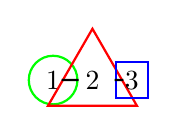
\begin{tikzpicture}\node[shape=circle,draw=green,align=center,line width=0.8pt] (0) at (0.5,10.166666666666666) {1};
\node[regular polygon,regular polygon sides=3,draw=red,align=center,line width=0.8pt] (1) at (1.0,10.166666666666666) {2};
\node[shape=rectangle,draw=blue,align=center,line width=0.8pt] (2) at (1.5,10.166666666666666) {3};

\path [-,draw=black,line width=0.8pt] (0) edge node {} (1);
\path [-,draw=black,line width=0.8pt] (1) edge node {} (2);
\end{tikzpicture}
\end{document}